\documentclass{article}\usepackage[]{graphicx}\usepackage[]{color}
%% maxwidth is the original width if it is less than linewidth
%% otherwise use linewidth (to make sure the graphics do not exceed the margin)
\makeatletter
\def\maxwidth{ %
  \ifdim\Gin@nat@width>\linewidth
    \linewidth
  \else
    \Gin@nat@width
  \fi
}
\makeatother

\definecolor{fgcolor}{rgb}{0.345, 0.345, 0.345}
\newcommand{\hlnum}[1]{\textcolor[rgb]{0.686,0.059,0.569}{#1}}%
\newcommand{\hlstr}[1]{\textcolor[rgb]{0.192,0.494,0.8}{#1}}%
\newcommand{\hlcom}[1]{\textcolor[rgb]{0.678,0.584,0.686}{\textit{#1}}}%
\newcommand{\hlopt}[1]{\textcolor[rgb]{0,0,0}{#1}}%
\newcommand{\hlstd}[1]{\textcolor[rgb]{0.345,0.345,0.345}{#1}}%
\newcommand{\hlkwa}[1]{\textcolor[rgb]{0.161,0.373,0.58}{\textbf{#1}}}%
\newcommand{\hlkwb}[1]{\textcolor[rgb]{0.69,0.353,0.396}{#1}}%
\newcommand{\hlkwc}[1]{\textcolor[rgb]{0.333,0.667,0.333}{#1}}%
\newcommand{\hlkwd}[1]{\textcolor[rgb]{0.737,0.353,0.396}{\textbf{#1}}}%

\usepackage{framed}
\makeatletter
\newenvironment{kframe}{%
 \def\at@end@of@kframe{}%
 \ifinner\ifhmode%
  \def\at@end@of@kframe{\end{minipage}}%
  \begin{minipage}{\columnwidth}%
 \fi\fi%
 \def\FrameCommand##1{\hskip\@totalleftmargin \hskip-\fboxsep
 \colorbox{shadecolor}{##1}\hskip-\fboxsep
     % There is no \\@totalrightmargin, so:
     \hskip-\linewidth \hskip-\@totalleftmargin \hskip\columnwidth}%
 \MakeFramed {\advance\hsize-\width
   \@totalleftmargin\z@ \linewidth\hsize
   \@setminipage}}%
 {\par\unskip\endMakeFramed%
 \at@end@of@kframe}
\makeatother

\definecolor{shadecolor}{rgb}{.97, .97, .97}
\definecolor{messagecolor}{rgb}{0, 0, 0}
\definecolor{warningcolor}{rgb}{1, 0, 1}
\definecolor{errorcolor}{rgb}{1, 0, 0}
\newenvironment{knitrout}{}{} % an empty environment to be redefined in TeX

\usepackage{alltt}

\title{An analysis of the television data set}
\author{Arthur Allignol}
\date{}
\IfFileExists{upquote.sty}{\usepackage{upquote}}{}
\begin{document}

\maketitle



We read the data using the follwing commands
\begin{knitrout}\scriptsize
\definecolor{shadecolor}{rgb}{0.969, 0.969, 0.969}\color{fgcolor}\begin{kframe}
\begin{alltt}
\hlstd{tele} \hlkwb{<-} \hlkwd{read.csv}\hlstd{(}\hlstr{"/data/Ulm/Teaching/SS_2014/Intro_Biostat_Comp/Illustrations/Television/data/television.csv"}\hlstd{,}
                 \hlkwc{stringsAsFactors} \hlstd{=} \hlnum{FALSE}\hlstd{,} \hlkwc{na.strings} \hlstd{=} \hlstr{"*"}\hlstd{)}
\end{alltt}
\end{kframe}
\end{knitrout}
and an excerpt of the data are displayed below.
\begin{knitrout}\scriptsize
\definecolor{shadecolor}{rgb}{0.969, 0.969, 0.969}\color{fgcolor}\begin{kframe}
\begin{alltt}
\hlkwd{head}\hlstd{(tele)}
\end{alltt}
\begin{verbatim}
##      Country life    tv phys fem male
## 1  Argentina 70.5   4.0  370  74   67
## 2 Bangladesh 53.5 315.0 6166  53   54
## 3     Brazil 65.0   4.0  684  68   62
## 4     Canada 76.5   1.7  449  80   73
## 5      China 70.0   8.0  643  72   68
## 6   Colombia 71.0   5.6 1551  74   68
\end{verbatim}
\end{kframe}
\end{knitrout}
\verb=Country= is the country name, \verb=life= is the life expectancy at birth, while \verb=tv= and \verb=phys= 
are the number of people of television set and the number of people per physicians, respectively.

\begin{knitrout}\scriptsize
\definecolor{shadecolor}{rgb}{0.969, 0.969, 0.969}\color{fgcolor}\begin{kframe}
\begin{alltt}
\hlstd{oldpar} \hlkwb{<-} \hlkwd{par}\hlstd{(}\hlkwc{no.readonly} \hlstd{=} \hlnum{TRUE}\hlstd{)}
\hlkwd{par}\hlstd{(}\hlkwc{mfrow} \hlstd{=} \hlkwd{c}\hlstd{(}\hlnum{1}\hlstd{,} \hlnum{2}\hlstd{))}
\hlkwd{hist}\hlstd{(tele}\hlopt{$}\hlstd{tv,} \hlkwc{main} \hlstd{=} \hlstr{"Number of people per TV"}\hlstd{)}
\hlkwd{hist}\hlstd{(tele}\hlopt{$}\hlstd{life,} \hlkwc{main} \hlstd{=} \hlstr{"Life expectancy"}\hlstd{)}
\end{alltt}
\end{kframe}\begin{figure}
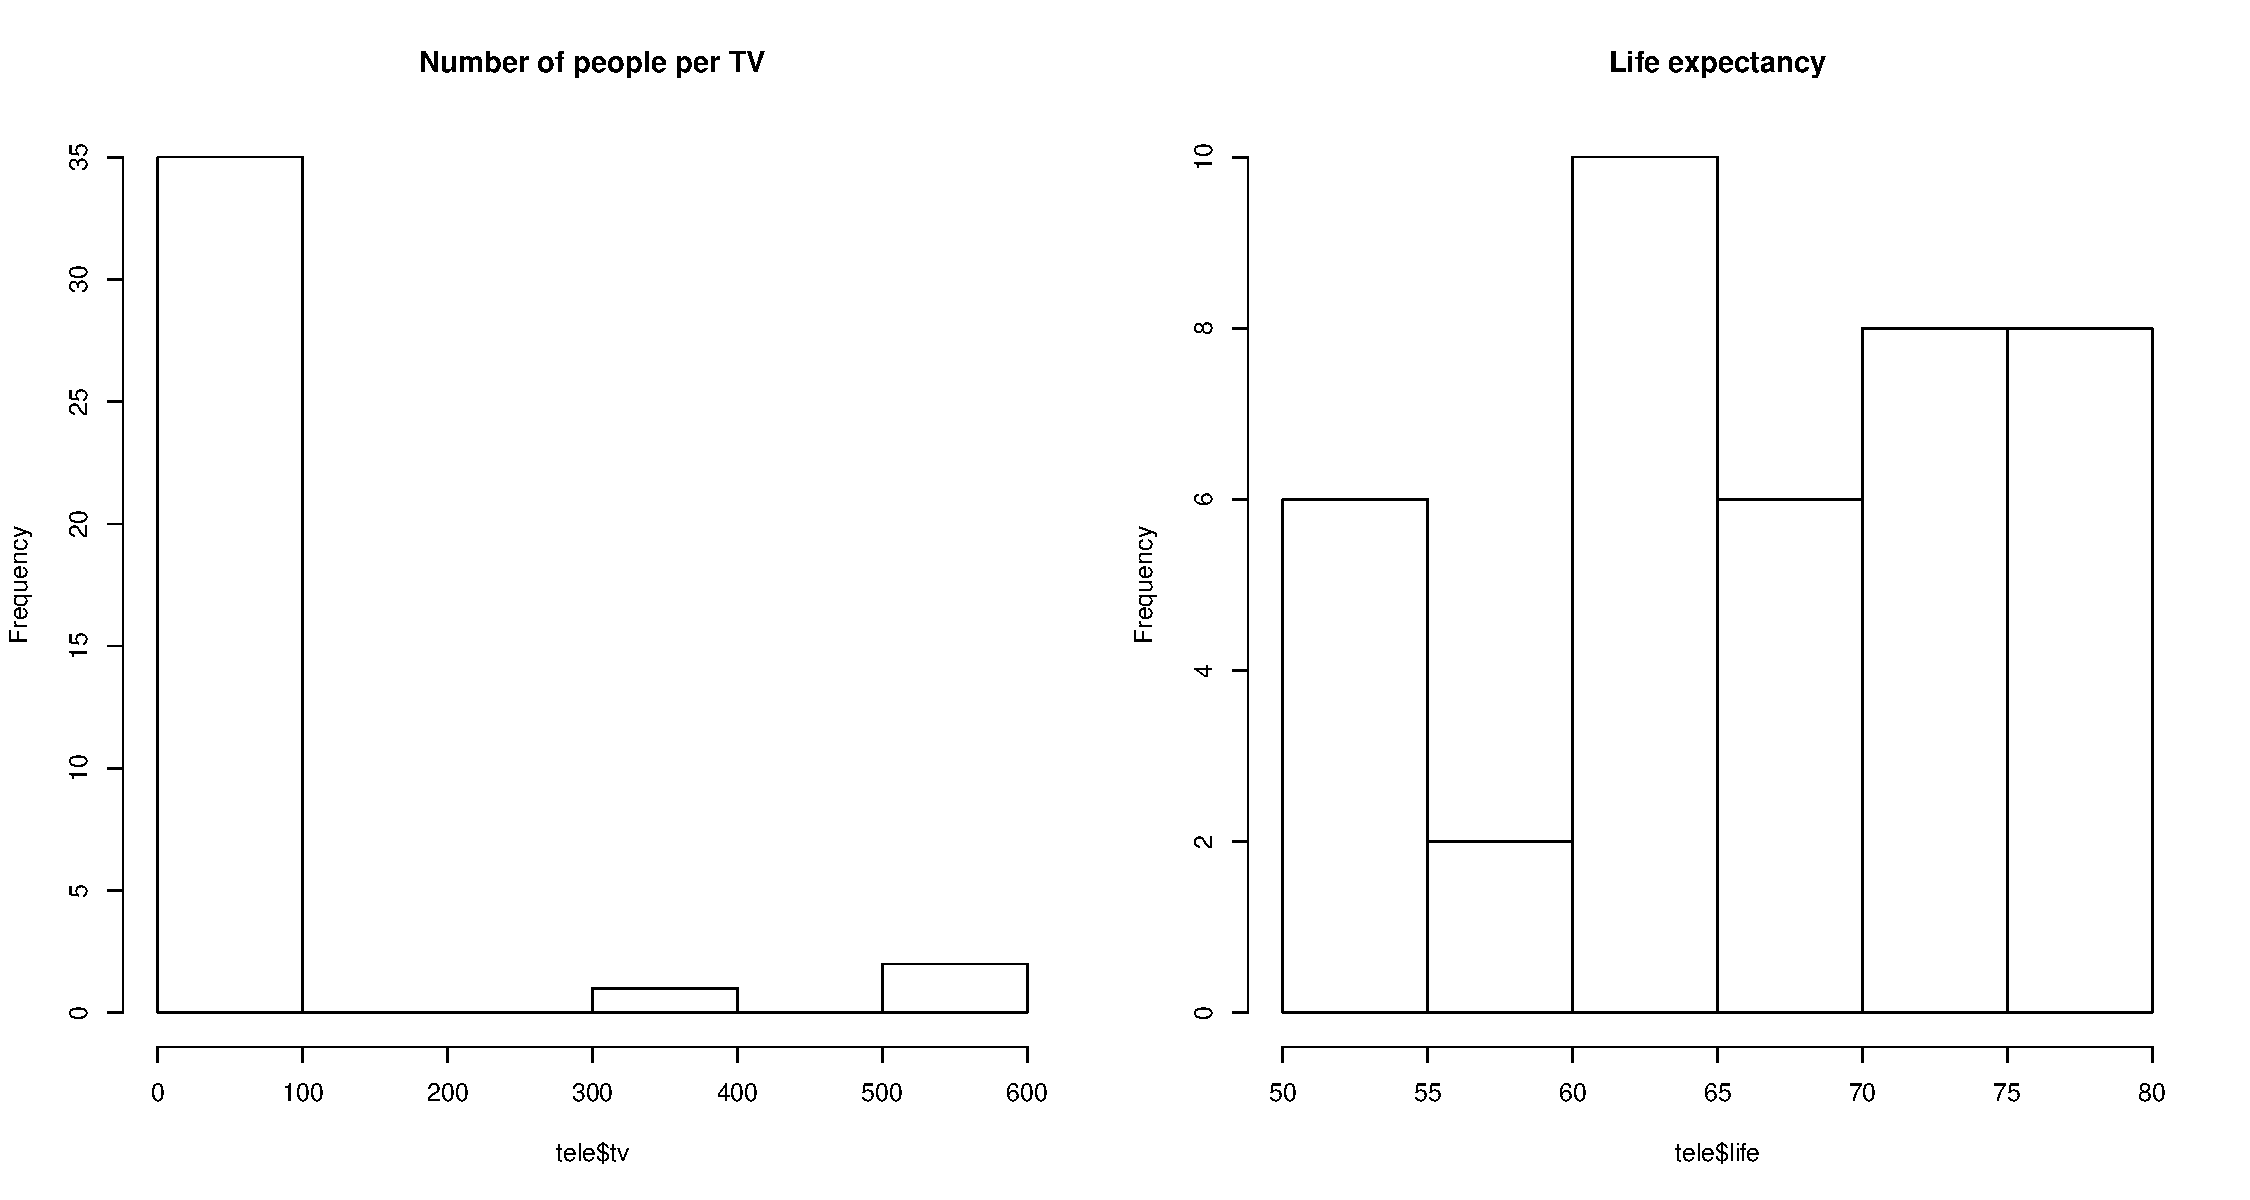
\includegraphics[width=0.7\textwidth]{graphics/unnamed-chunk-3-1} \caption[Histograms of {\tt tv} and {\tt phys}]{Histograms of {\tt tv} and {\tt phys}}\label{fig:unnamed-chunk-3}
\end{figure}

\begin{kframe}\begin{alltt}
\hlkwd{par}\hlstd{(oldpar)}
\end{alltt}
\end{kframe}
\end{knitrout}


\end{document}
